The following section explores the three popular graph querying languages -- two of which are used in the databases being investigated in this report -- and properties and techniques of graph querying. Graph querying languages have a notion of traversing the graph and accumulating results from pattern matching. This makes it very different to traditional SQL and is the main factor in contributing to the learning curve -- how to conceptualize graph expressions. These languages are still fairly new and there are many more being developed as the technique of graph traversal becomes more refined.

\subsection{Languages}
\label{subsec:lang}

\paragraph{Gremlin}

Gremlin is a functional, data-flow query language running on its own virtual machine \cite{gremlin-tinkerpop}. Due to how Gremlin is compiled, it can be written in both an imperative and declarative manner and be embedded into a host-language \cite{tinkerpop-docs}. Imperatively querying with Gremlin involves explicitly stating the traversal pattern whereas declarative allows the traverser to decide. The benefits of using an embedded querying language is that security risks from string concatenation and sanitizing input is handled automatically.

Gremlin integrates into multiple vendors (in our case, JanusGraph) and benefits from Turing-completeness. Each transaction is local to a given thread which means that a transaction is automatically created in that thread without having to explicitly call a create method. Transactions are atomic and support rollbacks.

\begin{figure*}[h]
    \centering
    \begin{verbatim}
        g.V().has("User", "user_id", "qUL3CdRRF1vedNvaq06rIA")
                .outE("REVIEWS").has("stars", gt(3)).order().by("date", desc)
                    .as("stars", "text")
                .inV().has("location", geoWithin(Geoshape.circle(35.15,-80.79, 5)))
                    .as("business_id")
            .select("stars", "text", "business_id")
            .by("stars").by("text").by("business_id")
    \end{verbatim}
    \caption{Returns all the reviews by the specified user ID within a 5km radius of 35\degree 15N 80\degree 79W ordered by date descending. The ability to query and index spatio-temporal properties is provided by JanusGraph's integration with a search engine such as ElasticSearch.}
    \label{lst:gremlin-example-1}
\end{figure*}

\paragraph{Cypher}

In an effort to create an easier graph language to pick up, Cypher (see the openCypher project \cite{opencypher}) was created as a very SQL-like query language. Unfortunately, while it is easier to pick up, it is not Turing-complete \cite{modern-graph-query-lang}. Use of ASCII-art helps to create more intuitive and easy to visualize queries e.g. edges are denoted by \verb|-->| or \verb|--[..]->| and vertices by use of parenthesis \verb|(b:Business)|.

Cypher is a declarative language so there is less control over how the traverser goes about each step. This means that Cypher has less flexibility and could perform worse when compared to Gremlin. Another criticism in terms of performance is that Cypher compiles into Gremlin which is then executed by the TinkerPop engine \cite{backtothefuture} and this overhead has yet to be optimized to where it should be when compared to traversal performance benchmarks. At the time of writing, Neo4j has been gathering more attention around Cypher, so the performance issues may improve significantly in the near future.

Cypher has the advantage of being able to express complex traversals in a simpler and more intuitive manner than Gremlin. Due to the open-source nature of Cypher and, how closely it is linked to Gremlin, it benefits from the same portability advantages by being able to integrate with multiple vendors. TinkerPop 3 supports Cypher\footnote{https://github.com/opencypher/cypher-for-gremlin} so any TinkerPop 3 enabled graph database can be queried with either language and benefit from both whether making a high-level traversal or simple query. An example of a useful query on this dataset can be seen in Figure \ref{lst:cypher-example-1}.

\begin{figure*}[h]
    \centering
    \begin{verbatim}
        CALL apoc.periodic.iterate(
            "MATCH (p1:User) RETURN p1",
            "MATCH (p1)-[:REVIEWS]->(r1)-->()<--(r2)<-[:REVIEWS]-(p2)
                WHERE id(p1) < id(p2)",
            {batchSize:100, parallel:true, iterateList:true}
        );
    \end{verbatim}
    \caption{Returns all users who have reviewed the same businesses as a given user. This iterates through all of the users. Note how the return match checks that the user \texttt{p1} does not match user \texttt{p2}.}
    \label{lst:cypher-example-1}
\end{figure*}

\paragraph{GSQL}

GSQL is described as a SQL-like language which is the conceptual descendent from technologies such as Gremlin, Hadoop MapReduce, SQL, Cypher and SPARQL \cite{gsql-tigergraph}. GSQL, like Gremlin, is a Turing-complete graph query language that accumulates data along a traversal. One limitation that Gremlin has over GSQL is that Gremlin cannot simultaneously group two tables by separate group-by attributes. GSQL achieves this by providing the ability to define multiple grouping accumulators.

In GSQL, there is a large emphasis on creating a language that enables massively parallel processing on queries. The vertex and edge blocks in GSQL queries indicate independent computations separated by incoming vertices or edges referred to as guarding conditions. These blocks are pieced together by the output of one block being the input of another. Control of this flow can be handled by if-then-else or while statements allowing for subsequent blocks using dynamically calculated input.

As with Gremlin, there is an emphasis on a strong, functional programming style. One has the ability to define named, parameterized queries which is analogous to creating a function with arguments. These parameterized queries can then be called by other queries enabling the re-use of code. As is the case with Gremlin and Cypher, TigerGraph allows for the conversion of Cypher to GSQL for those migrating from their competitor, Neo4j \cite{tigergraph-infoworld}.

\textcolor{blue}{TODO: Show examples of GSQL}

\subsection{Graph Pattern Matching}

Graph pattern matching is an example of \emph{declarative} (descriptive) querying. Basic graph patterns follow the structure of the graph to query. A basic graph pattern for a property graph\footnote{Which is the type of graph being investigated in this paper.} is a graph where variables appear on the edges and vertices. A \emph{match} for a basic graph pattern is then mapped against the graph being queried. The variables in the basic graph pattern subgraph is matched to selected values or constants in the original graph and returned as a result \cite{foundations-of-modern-gql}. An example of the pattern produced by Figure \ref{lst:gremlin-example-1} can be seen in Figure \ref{fig:gremlin-pattern}.

\begin{figure*}[h]
    \centering
    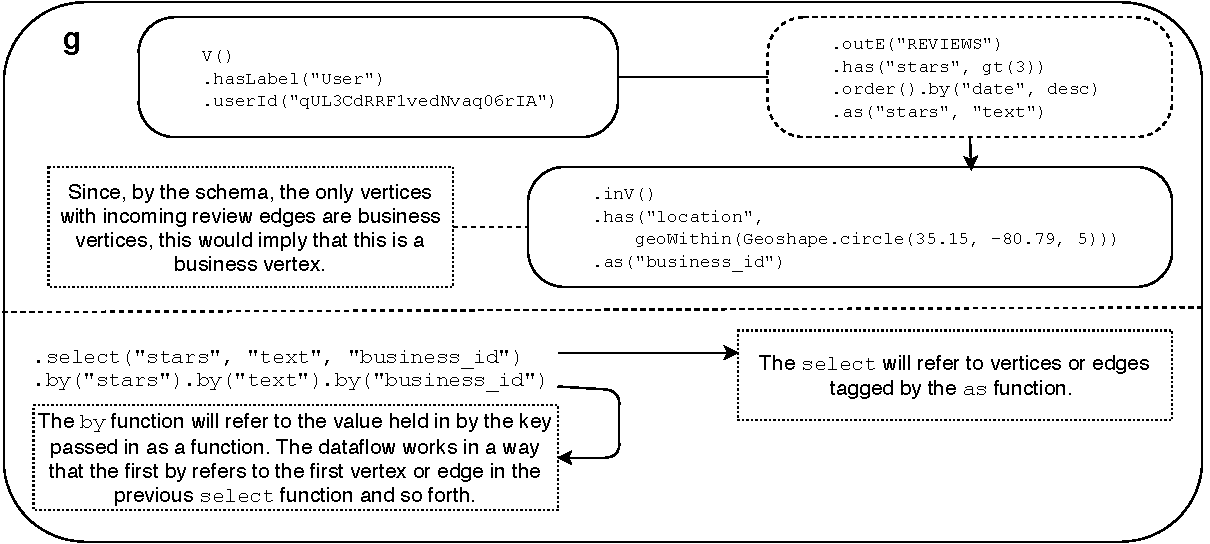
\includegraphics[width=16cm]{img/gremlin-pattern.pdf}
    \caption{An illustration of the graph pattern produced by Figure \ref{lst:gremlin-example-1}. The top half shows the graph traversal pattern and the bottom half how the output is projected from the matched vertices and edges.}
    \label{fig:gremlin-pattern}
\end{figure*}

Complex graph patterns extend on basic graph patterns by including the traditional relational operators used for sets such as union, difference, optional, and filter. These operators are described as follows:

\paragraph{Projection} A projection returns a subset of data from the accumulated results of the pattern match. An example of this is to return only the stars from reviews between a user and business and exclude the text and edge IDs.

\paragraph{Join} The join of two basic graph patterns corresponds to the function of a natural join in classic relational query languages such as SQL. Since the output of a basic graph pattern is the result of the variables specified on the graph pattern, the output of a join between two basic graph patterns is the union of their output variables.

\paragraph{Union and difference} The union of two basic graph patterns is satisfied when one pattern or the other satisfies the pattern match. The difference of two basic graph patterns where the set of matches in the one are not in the set of matches in the other.

\paragraph{Optional} Optional works much the same as \emph{join}, but instead of discarding the results from the evaluation which cannot be joined, the results from both matches are kept. This allows data with incomplete or unavailable properties to remain in the output.

\paragraph{Filter} The filter operator restricts the matches over which the traversal is performed. In practice, these filtering criteria vary in complexity with the ability to search over regular expressions (when querying string data), between dates (when querying temporal data), and over a radius (when querying spatial data).

\subsection{Navigational Queries}

Angles, et. al. \cite{foundations-of-modern-gql} describes navigational queries as queries where the length of the traversal is potentially arbitrary such as \emph{path queries}. Path queries are the most basic navigational queries, where one is only interested in the results accumulated when traversing from a source to a destination. Path queries are useful when looking at friend-of-a-friend relations between users in social networks and find applications in route-finding \cite{route-finding}.

An example of one such query can be seen in Figure \ref{lst:cypher-nav-1} and \ref{lst:gremlin-nav-1}.

\begin{figure}[h]
    \centering
    \begin{verbatim}
    MATCH (x1:User) -[:friends*]-> (x2:User)
    RETURN x1, x2
    \end{verbatim}
    \caption{Simple friend-of-a-friend query written in Cypher.}
    \label{lst:cypher-nav-1}
\end{figure}

\begin{figure}[h]
    \centering
    \begin{verbatim}
    g.V().hasLabel(`User')
            .out(`FRIENDS')
         .hasLabel(`User')
    \end{verbatim}
    \caption{Simple friend-of-a-friend query written in Gremlin.}
    \label{lst:gremlin-nav-1}
\end{figure}

Navigational queries that try to match no-repeated-node or edge paths problems are typically NP-complete. Due to this, it is often necessary to add additional limitations on the pattern to be matched or use imperative querying techniques. Another common path traversal includes shortest paths from one vertex to another or path existence queries. It is evident how the complexity of path traversals can be so it becomes increasingly important to bound these types of queries using tools such as \texttt{repeat...times(x)} from Gremlin to limit the search space of these types of queries.
